%%%%%%%%%%%%%%%%%%%%%%%%%%%%%%%%%%%%%%%%%%%%%%%%%%%%%%%%%%%%%%%%%
%%%%%%%%%%%%%%%%%%%%%%%%%%%%%%%%%%%%%%%%%%%%%%%%%%%%%%%%%%%%%%%%%
%%%%%%%%%%%%%%%%%%%%%%%%%%%%%%%%%%%%%%%%%%%%%%%%%%%%%%%%%%%%%%%%%

\chapter{Introduction to Programming in Java}
\label{chap:IntroJava}

%%%%%%%%%%%%%%%%%%%%%%%%%%%%%%%%%%%%%%%%%%%%%%%%%%%%%%%%%%%%%%%%%
\section{Programming in Java}
\label{sec:Programming}

It is clear that it is not possible to teach simulation methods without 
performing some numerical experiments in the classroom and that it is 
impossible for the students to learn stochastic simulation methods without 
implementing the algorithms. Therefore, the theory and the corresponding 
algorithms will be presented in a highly interconnected, and, we 
hope, organic way.



\subsection{Reasons for Choosing Java ?}
\label{sec:Programming_languages}

In order to stick to this idea it was necessary to choose a programming 
language or a tool, which makes realizing a simulation algorithm
easy. The obvious criteria for taking such a decision are
\cite[]{GARCIA}
\begin{description}
\item[Efficiency] How much work has to be done to realize a given
        simulation algorithm on a computer and gather results, maybe
        visualize them ? \newline 
        What tools are available to aid in this process ? \newline
        What has to be done to use standard mathematical capabilities
        like 
\begin{itemize}
\item Statistics (mean, std. deviation, probability distributions, etc.)
\item Transformations like FFTs, Filters, etc.
\item Approxmiations (nonlinear equations, etc.)
\item Parameter Estimations like least square method, etc.
\item Interpolation and Integration of functions
\item Solving ODEs and PDEs
\item using matrices and arrays
\item random number generation for different PDFs
\item computing with complex numbers
\end{itemize}
\item[Understandability] Structured or object oriented language ? \newline
        Bad programming style possible or not ? \newline
        Documentation freely available ? \newline
        Is it possible to generate documentation directly from the
        source code ?
\item[Graphical Capabilities] How to visualize data (Plots, 2D, 3D, 
        line graphs, log-log plots, bar graphs, surface plots, vector 
        plots, etc.) \newline
        How difficult is it to realize GUIs ? (needed to watch reactions
        of the system by changing environmental conditions / parameters.)
        \newline
        Is it possible to produce EPS graphics output for later use
        in documentations, papers, etc. ?
\item[Standard / Portability] Does the produced computer simulation scale
        from a small computer, maybe a PC, up to large high performance
        massivley parallel computers ? \newline
        Independence of the underlying operating system, computer hardware
        and even the physical place of the computer. 
\item[Cost / License] What has to be paid to get a development environment
        for a student ? \newline
        Is the software / tools under the GNU license ? \newline
        Is the produced code / simulation reusable (e.g. a clean 
        object oriented aproach is usually better reusable than a structured
        approach.) ?
\item[Performance / Parallelizability] How long does the simulation run
        on a given computer ? \newline
        How large (=resources) 
        does the computer have to be to get reliable results ?
\item[Reproducability] Is the language / tool usable for everybody to
        reproduce / confirm the results ? \newline
        Are all tools / programs open source, so that everybody can
        take a look inside and confirm the correctness of the 
        computations ? \newline
        Tests must be applied and results are verified.
\end{description}

An aim of the course is to make the student acquainted with a 
programming language ``in action'' so they should learn something 
about a ``good 
programming style'' for real-life problems. Writing clean software 
efficiently is important for a physicist to 
concentrate on physically relevant topics and to produce reproducable 
results, which can be verified later by anyone in the world.

Visualization of the results 
obtained allows to understand more easily what is going on physically. So 
the interface between program and visualization tool/graphical output should
be comfortable. Last but not least the availability of the program should be
guaranteed. The corresponding compilers should be available at low, in the 
ideal case at no cost to the students for home exercises. Furthermore, they
should be portable on PCs with Windows or Linux operating systems, on Macintosh
and on workstations from the UNIX world (IBM AIX, Solaris, SGI Irix, ...).
Since almost all universities do have a high--performance parallel computer 
the language should also allow to demonstrate high--performance parallel 
algorithms and designs.

Because of our background of convinced Fortran users we considered the 
following alternatives: 
\begin{itemize}
\item programming languages 
 \begin{itemize}
  \item Fortran
  \item C
  \item C++
  \item Java
 \end{itemize}
\item modern script languages
 \begin{itemize}
   \item Python
 \end{itemize}
\item higher level mathematical tools
 \begin{itemize}
   \item Matlab
   \item Octave
 \end{itemize}
\item symbolic mathematical packages
 \begin{itemize}
   \item Maple
   \item Mathematica
 \end{itemize}
\end{itemize}

All the languages considered  in some sense satisfy the above criteria. All
are more  or less portable on different platforms (at different expenses), all
allow the use of good visualization tools (at different prices), and, of 
course, all are mostly clean. But not all are equally powerful. 

To get a better impression on how the different possibilities fit into 
our requirements, we have put together a table, which shows the
ratings for the different requirements for each of the considered 
solutions.

\begin{landscape}
\begin{table}[htbp]
\begin{tabular}{|c|p{1cm}||p{2cm}|p{2cm}|p{2cm}|p{2cm}|p{2cm}|p{2cm}|p{2cm}|}
\hline
Language / Tool & Avg. Points &
Efficiency & Under\-standa\-bility & Graphical Capabilities &
Standard / Portability & Cost / License & Performance / Parallelizability &
Reproducability \\\hline
C          & 4.9 & 6 & 3 & 3 & 4 & 7 & 9 & 2 \\\hline
C++        & 5.6 & 7 & 5 & 3 & 5 & 7 & 7 & 5 \\\hline
Fortran 95 & 5 & 6 & 4 & 1 & 7 & 3 & 9 & 5 \\\hline\hline
Java       & 8.0 & 8 & 8 & 7 & 8 & 9 & 7 & 9 \\\hline
Python 2.2 & 7.7 & 8 & 7 & 6 & 8 & 9 & 8 & 8 \\\hline\hline
Matlab 5.2          & 5.1 & 8 & 7 & 9 & 3 & 1 & 4 & 4 \\\hline
Octave 2.0.16       & 5.7 & 8 & 7 & 5 & 3 & 9 & 4 & 4 \\\hline\hline
Maple / Mathematica & 3.6 & 5 & 3 & 8 & 3 & 1 & 2 & 3 \\\hline
\end{tabular}

\caption{On a scale from 1 to 10, where 10 is perfect and 1 is very bad.
The results are due to the underlying question: How does the tool / language
perform for realizing a stochastic simulation algorithm on a computer.}
\end{table}
\end{landscape}

Because some of the later introduced simulations are very time consuming,
we also checked the performance of the solutions considered by the 
following benchmark, which represent the prototype of a stochastic simulation. 
We generated 100 trajectories of a typical one-step stochastic process
(see Chapter \ref{sec:OneStepProcesses})
and compared the CPU times obtained by different languages. The result
of the benchmarks are summarized in the following table \ref{tab:Performance}. 
The listings
of the corresponding programs are listed in the appendix.

\begin{table}[htbp]
  \begin{center}
    \leavevmode
    \begin{tabular}{llp{3cm}|c|c}
      Language & OS & Software & Machine & CPU time \\\hline\hline  
   Fortran 90 & Linux & Nag f90 Compiler V2.2(260) & Pentium 133 & 2.1 sec.\\
           & Linux & Nag f90 Compiler V2.2(260) with -O3 & Pentium 133 & 2.4 sec.\\
           & Linux & Nag f95 Compiler V1.0(436) & Pentium 133 & 2.3 sec.\\
           & Linux & Nag f95 Compiler V1.0(436) with -O4& Pentium 133 & 2.3 sec.\\
\rowcolor{tabgray} & Linux & Pallas f95 Compiler V3.0-3 & Pentium 133 & 1.3 sec.\\
           & Linux & Pallas f95 Compiler V3.0-3 with -O4& Pentium 133 & 1.4 sec.\\\hline
   C       & Linux & GCC 2.7.2.3 & Pentium 133 & 2.1 sec. \\
\rowcolor{tabgray} & Linux & GCC 2.7.2.3 with -O3 & Pentium 133 & 2.0 sec. \\\hline
   C++     & Linux & egcs-1.0.3 & Pentium 133 & 2.2 sec. \\
           & Linux & egcs-1.0.3 with -O3 & Pentium 133 & 1.8 sec. \\\hline
      Java & Linux & JDK 1.1.7, no JIT & Pentium 133 & 16 sec. \\
\rowcolor{tabgray} & Linux & JDK 1.1.7, with JIT TYA (V1.3) & Pentium 133 & 10 sec.\\
           & Linux & JDK 1.1.7, no JIT & DEC Alpha 21164 600 & 6 sec. \\
           & Win95 & JDK 1.1.7, with Symantec JIT & Pentium 133 & 9 sec. \\
           & Win95 & JDK 1.1.7, no JIT & Pentium 133 & 19 sec. \\
\rowcolor{tabgray} & Win95 & JDK 1.2, with Symantec JIT & Pentium 133 & 8 sec. \\
           & Win95 & JDK 1.2, no JIT & Pentium 133 & 22 sec. \\\hline
   Matlab  & Win95 & Matlab 5.1 & Pentium 166 & 330 sec.\\
\rowcolor{tabgray} & Win95 & Matcom Compiler V3.0 with Borland C++ 5 & Pentium 166 & 70 sec.\\
           & Linux & Matlab 5.2 & Pentium 133 &  224 sec.\\\hline
   Maple   & Linux & Maple V Rel. 4 & ??? & \\\hline
Mathematica& Win95 & Mathematica V3.0 & Pentium 133 & 28 Min. \\
\rowcolor{tabgray} & Win95 & with Compiler    & Pentium 133 & 26 Min. \\ \hline
    \end{tabular}
    \caption[Performance Table.]%
    {Performance comparison for different languages, operating
      systems (OS), and platforms.
      The test program is a one-step stochastic process. We create 100
      realizations, $g(n)=0.4n, r(n)=0.5n$ (see Chapter 
      \ref{sec:OneStepProcesses}).
      On Windows 95 the JIT from
      Symantec is included and automatically used, when executing programs
      with the java command in the JDK. The TYA JIT for Linux is freely
      available and easy to install. Usage: with the Java virtual machine of
      the JDK use \texttt{-Djava.compiler=tya} or 
      set the environment variable \texttt{JAVA\_COMPILER=tya}. To avoid
      using the JIT use option \texttt{-nojit} up to JDK1.1.7 on Windows or
      for all other platforms set the environment variable 
      \texttt{JAVA\_COMPILER=none}.
      }
    \label{tab:Performance}
  \end{center}
\end{table}


Of course, in the above test we have neither optimized the algorithm nor
the implementation to the 
different platforms. Nevertheless, the table clearly shows that 
symbolic Math packages and higher level math languages are 
very slow. Even the compiled version of MATLAB is slower by a factor of 
about 100 
compared to the Fortran code. This is a good reason to disregard 
these solutions for our purposes.

Now we have to decide between the programming languages and the scripting 
languages. The argument in favour of 
Java which compensates the slightly slower performance (today!, in future 
this might be different) is its portability and the free availability of the
compiler, the GUI capabilites coming with the standard language package
and of the visualization tools. Java runs on every platform and 
it is available at no cost. 

With Java, we do not even have to change any line
of code to get a faster performance, because we just have to get a faster
Just in Time compiler or a JIT with the HotSpot technology, which improves
performance by factors of 2 to 10 or even more. This will free the
programmer from time consuming and difficult optimizaions. 
There is also for example a compiler called High Performance Java by IBM. It generates
much faster code on IBM workstation compared to the JDK from SUN and the 
speed is already comparable to C/C++. 
For a comparison with this compiler see \cite[]{HPJ}.

Last but not least, we want to mention a further advantage of Java. It seems
\cite[]{bigbucks} that there is  a great need for Java programmers in 
various branches of industry today. This need will even grow in future 
years. So learning Java might be a kind of ``life insurance'' for students of 
physics. It will put them in the position to find a good  job in the
software industry.


%%%%%%%%%%%%%%%%%%%%%%%%%%%%%%%%%%%%%%%%%%%%%%%%%%%%%%%%%%%%%%%%
\subsection{Java}
\label{sec:Java}

In Chapter \ref{sec:Programming_languages} we have given
some good reasons to choose Java as the programming language
for our purposes. Here we want to mention some more technical points, from a 
computational science point of view, in favour of Java. Some of the points
are very technical and are only be understood with knowledge about
pogramming. So for beginners it might be useful to come back again here
after learning Java in the next chapters.

SUN Microsystems has described Java as follows \cite[]{javanutshell}:
\begin{quote}
Java: A simple, object--oriented, distributed, interpreted, robust, secure,
architecture neutral, portable, high--performance, multi-thread, and dynamic 
language.
\end{quote}
Let us try to understand roughly what is meant by the above adjectives.

Java is simple in the sense that the number of language constructs has been 
kept as small as necessary. For ease of migration from other languages some
basic language elements resemble C or C++. However, some features of these 
languages which were rarely used and which have been considered to be unsafe 
have been omitted. For example, in Java there is no \verb|goto|
 statement; instead 
it has labelled break and continue statements. The preprocessor of C has been 
eliminated; the program you write is the program that the compiler sees. In 
Java there are no  operator overloading and no multiple inheritance 
features known from C++. But you can use interfaces to simulate 
multiple inheritance and argument overloading is also possible.
One major simplification is that Java does not have pointers!
In Java memory is taken care of automatically, so the programmer is not responsible 
for the memory management. In particular, Java implements an 
automatic  garbage collector.

Java is an object--oriented language and you do not have to think in a 
procedural--based way, as it is the case in Fortran for example. In order to 
solve problems in Java we are forced to use the notions of classes and objects. 
Every object has a class that defines its data and the methods that operate 
on these data. Classes are hierarchically arranged. A subclass inherits the 
behaviour of its superclass. A class is the basic unit of compilation
and of the execution in Java. All Java programs are classes.
Of course you do not have to use the object oriented programming style,
you can still stick to the procedural style in Java too.

Java is a distributed language, which simply means that it provides a lot of 
tools for networking. Java is the programming language of the Internet.

Java is an interpreted language. The Java compiler compiles the Java
source code into Java byte--code, which is the machine language for the Java
Virtual Machine (JVM). The JVM is an abstract machine which runs on each system
that supports Java. Programs written in other languages 
may also be compiled into Java byte-code.

Java is robust. Java contains a feature, called 
exception handling, which simplifies the
task of error handling and recovery.

Java is secure. Since Java has been designed for distributed applications
high security standards have been implemented. For example, direct access to
memory is not allowed. Java contains four different levels of security 
checks and enforcements to prevent the introduction of viruses. 
In particular there is protection against deleting and modifying files.

Java is architecture neutral and portable. The byte-code format is always the 
same regardless of the platform on which the Java compiler runs. Furthermore,
there are no ``implementation defined'' behaviours in Java. For example, Java
specifies the size of each primitive data type. The integer 
types byte, short, int, long take 8, 16, 32, 64 bit of memory, respectively.
This also avoids the use of any preprocessor available to all other
languages, excessively used in C and C++ to catch all
platform relevant parameters.

Java is a high--performance language. 
Usually Java is run using an interpreter, the so-called  Java Virtual Machine.
It is however possible to run Java with a 
Just In Time (JIT) compiler, which translates the bytecode to native code
before the code gets executed. JIT compiling increases the performance of Java 
considerably.

Java is multi-threaded. It supports multiple threads of execution which can 
handle different tasks. Multi-threading increases the interactive performance 
of Java.

Java is dynamic. Any Java class can be loaded into a running Java interpreter 
at any time.

Java includes the zlib compression library in the 1.1. language specification.
These are
the freely available compression libraries used in the well-known
gzip compressor.
That makes it very easy to write and read compressed data. 


\subsection{Brief History of Java}
Java started off in 1991 as a project by James Gosling, which at that 
time was called
Oaks. Its purpose was focussed on the use as operating  
software (OS) for consumer
electronic devices. A small group decided to adapt Oak to web
technology and released the first version of Hotjava (a web browser, at that
time still called WebRunner)
in late 1994. After a presentation given by James Gosling about the 
byte codes used by Oak in 1995, the new language JAVA was officially 
announced in April 1995 (Java 1.0), 
including the first official release of Hotjava.
The announcement was the source of a hype, because Java is ideally
suited for the heterogenous world of networked computers seen today and
the Java philosophy allows for ``Write Once, Run Everywhere'' including
graphical capabilities.

Then in January 1996 the first version of the Java Development Kit (JDK) 
was released by SUN. Soon the language was licensed by many companies,
most notably Netscape, which included a Java Virtual Machine (JVM) into
their widely used browser Netscape Navigator. Then in early 1997
SUN released the second version of Java: the new language specification 
Java 1.1 and the development kit for it, JDK 1.1.

Meanwhile most of the browsers adapted the new Java 1.1 language specification.
Also many new APIs (Application Programmers Interfaces) like Java 3D or 
most important the JFC\footnote{The Java Foundation Classes, which
consist of the Swing API and many more components like (an 
almost complete set of)  
the Internet Foundation Classes (IFC). You can either use Java 1.1 together
with the JFC 1.1 for Swing 1.1 or Java 2, which already includes JFC 1.1 for
Swing 1.1 and also Java 2D and some more new APIs.}
have appeared, some
of them have been officially included in the Java 1.2 specifications
(now called Java 2). Together with the JDK 1.2, Java 2 appeared in January 1999.
But no browser supports this standard right now, although most
of the software available for Java and written in Java seem to be
already adapted to the new standard. Another change occurred to the
licensing of the JDK: it is now almost Open Source Software, which
means you can have the source code and change it, you only have to make
sure it still conforms to the Java standard.

At the same time SUN released a new project called JINI, which is
a ``small set of instructions and interfaces'' based on Java to
be used to drive and use arbitrary electronic devices in a local network--
the actual aim of the Oaks/Java project started in 1991. The idea is that every 
JINI device reports to a ``naming service'' and tells it, what services
it provides to the network. The server can then tell, what services are
available at all to somebody at some place. Therefore the device can be 
taken to any place in the world and used in any JINI network to which
it can connect. You do not even need a JVM in the device, you can 
use a JVM supplied by a different device (e.g. a computer or browser) 
available in the network. The whole system is based on Java code and
the RMI protocol supplied by Java.

%%%%%%%%%%%%%%%%%%%%%%%%%%%%%%%%%%%%%%%%%%%%%%%%%%%%%%%%%%%%%%%%%%%%%
\subsection{SUNs Java Naming Scheme}
\label{sec:NamingScheme}
SUN introduced a new naming scheme for the Java versions in 1999. So there is a 
version number referencing the language version and a version number
referencing the API kit coming with the JDKs released by SUN.
They call all the Java Language specifications refering to the JDK versions
1.x.x as Java1 and the JDK versions 1.2.x up to 1.4.x are called Java2.
But sometimes people refer to the JDK version directly instead of
refering the Java language version, which sometimes makes it difficult to
follow. So we adopt the SUN language and will explicitly state, if we
refer to the JDK version or the Java Language version 1 or 2
(see also table \ref{tab:JavaNamingScheme}).
\begin{table}[htbp]
  \begin{center}
    \leavevmode
    \begin{tabular}{llp{3cm}|c|c}
      Java Language Version & SUN JDK Version & Approx. Release Dates \\\hline  \hline
	Java 1 & JDK 1.0 & ??? \\\hline 
	       & JDK 1.1 & ??? \\\hline 
	       & JDK 1.1.8 & ??? \\\hline 
	Java 2 & JDK 1.2.2 & ??? \\\hline 
	       & JDK 1.3.1 & ??? \\\hline 
	       & JDK 1.4 & February 2002 \\\hline 
    \end{tabular}
  \label{tab:JavaNamingScheme}
  \end{center}
\end{table}

%%%%%%%%%%%%%%%%%%%%%%
\section{Tools for Writing and Using Java}
\index{tools for Java}

Although we are describing many different programs in this chapter, the only 
necessary tools to work out the programs in this book are the JDK, an editor
like Emacs/XEmacs maybe with JDE and a WWW browser like Netscape or
Internet Explorer. 

\subsection{Programs:} 
\begin{description}
\item[JDK] \index{JDK} The Java Development Kit, distributed freely by SUN.\\
        This kit is available for almost all platforms, e.g. Windows,
        Solaris, Macintosh, Linux, etc. This is the first package to get,
        to use Java. It consists of a Java compiler, a virtual machine 
        and a debugger. There
        are of course many other compilers, JVMs and debuggers
        available, but this is the program to start with. A disadvantage
        of the JDK especially for Windows user is, that you have to use the
        command line to use it. There are no graphical interfaces  coming with the
        package to start, compile or debug Java programs.
        For Linux there is  a seperate package available, which contains
        the threaded versions for the JDK 1.1. This is mostly not
        included in the standard packages for the Linux distributions.
\item[MRJ/SDK] \index{MRJ} Apple develops the Java developement kit for the Macintosh and
  distributes two versions: the MRJ runtime environement (in version 2.0 included
  in MacOS 8.5 and the new version MRJ 2.1.2 from \href{http://developer.apple.com/java/}%
  {http://developer.apple.com/java/}) and the SDK for Macintosh in version
  2.1 as of the time of writing also available from the address above. These are
  versions supporting Java 1.1.7 and Swing/JFC. The new version MRJ 2.2
        is just getting available.
\item[Jikes] \index{Jikes} 
  Jikes is a Java compiler developed at IBM fully conforming
  to the Java specifications. It is free and much faster than most
  other compilers. Thy byte code produced is only slightly different.
  It is a nice replacement for the javac compiler of the JDK.
\item[Kaffe] \index{Kaffe} \href{http://www.kaffe.org/}{Kaffe} 
  is an open source 
  JVM. It is a replacement for the java JVM of the JDK. In version 1.0 it is
  already almost fully Java 1.1 compatible and it includes some of the
  Java 2 features. It runs under Windows and Unix systems. There is also
  a commercial version of Kaffe sold by 
  \href{http://www.transvirtual.com}{transvirtual}. This project unfortunately
  has not seen significant progress in the last year.
\item[GCJ] \index{GCJ} This is the 
  \href{http://sourceware.cygnus.com/java/gcj.html}{GNU compiler for Java}. 
  It can compile java
  source code files inot class files (bytecode) and it can even
  compile class files or source files directly into executable
  files on the platform running GCJ. GCJ is actually a front end
  to the free famous GCC/EGCS compiler suite. To compile class files
  to object code you also need the libgcj runtime library.
 ??? Version 3.0 ???

\item[CJ/GJ] \index{CJ} \index{GJ}
  \href{http://wwwipd.ira.uka.de/~pizza/gj/}{GJ}
  is an extension to the Java language that supports
  generic types. This can be used to for example to add primitive
  complex types to Java. This has been already done and the project
  is called \href{http://wwwipd.ira.uka.de/~gunthner}{CJ}. 
  The idea is to translate the Java source code including
  the generic types like the primitive complex type to pure Java 1.1
  or Java 1.2 code and then compile it with any Java compiler available.
  This approach is considered by SUN to become a standard approach
  for handling generic data types like complex numbers 
  in the JDK versions 1.4.x or 1.5.
\item[Jolt] The \href{http://www.redhat.com/}
  {JOLT - Java Open Language Toolkit} - Project. Tries to
  compose a full freely available Java developement kit. Should
  include kaffe, guavac and more.
\item[Emacs/XEmacs] \index{Emacs}\index{XEmacs}
  This is an editor available for most platforms.\\
  We basically use this very powerful but sometimes confusing
  editor to do all our programming, text editing and more. It is
  also available for Windows, but it is mostly used on UNIX machines.
  We are using the Emacs/XEmacs editor throughout the book, but 
  there is no restriction to any of the programs or examples, if
  you use a different editor.
\item[mpEdit] \index{mpEdit} A freely available editor written completely in Java and
  therefore available on all platforms.\\ 
  It has all necessary features to write Java/C or C++ programs.
\item[JDEE] \index{JDE} JDEE (Java Development Environment Extension) 
  is an Emacs/Xemacs extension
  written in Elisp. \\
  It enables you to write Java code in a shorter time, if you are
  using the emacs or xemacs editor. It is almost a complete environment for
  developing Java programs with emacs.
\item[Netscape Navigator/Communicator] \index{Netscape}
  A web browser like the Internet 
  Explorer, but written by Netscape inc. and the source code is
  freely available and fully conforming to the Java standard. \\
  We used Netscape and the appletviewer of the JDK to test all
  the applets in this book.
  Be aware that not everything is supported by all browsers and
  sometimes you get different results or the browser crashes,
  although the program did run with the appletviewer.
\item[Netbeans]\index{Netbeans} A commercial IDE for Java written in Java \\
  This is an object oriented IDE for Java. It is free for academic and 
  personal use, but not for commercial use. It has been bought by SUN
  in 2000.
\item[Simplicity for Java] \index{Simplicity for Java}
  A commercial IDE for Java written in  Java\\
  A very nice and easy to use IDE for Java. It is very easy to get started
  with it. It can even write event handling code for your 
  graphical user interfaces (GUI). Free trial versions are available
  from the \href{http://www.datarepresentations.com/}{homepage for Simplicity}.
\item[Fortran to Java / Harissa] \index{Fortran to Java} A Fortran 77 to Java Compiler. \\
  You can convert very easily Fortran 77 programs to Java. This is a part of the
  ``Java Access to Numerical Libraries'' project at the University of 
  Tennesee in the US. F2j was already capable of translating the
  Lapack routines to Java.
\item[Ant (Jakrata Project)] Ant is a replacement for make for Java programs.
  It is much easier to use and to set up for Java programs than make.
  It is used for the ``make'' process of the project you develop, because many
  projects not only consist of one or two files, but you have to take care
  of many files and directories.
\item[Lava Rocks] This is a ``free'' tool to resemble the behaviour of the
  well known C/C++ printf/scanf functions in Java. Sometimes it can be handy
  to use it.
\end{description}

\subsection{Java Packages:}
All these packages are used extensivly throughout this book and they
are recommended for own Java projects. For most of the programs
presented in this book, you have to install these packages.
\begin{description}
\item[simulation] \index{simulation package} ??? (mehr Werbung)
  This is the package developed during the writing
        of this book. It provides some basic features, which
        might be of interest or can ease writing code. All the missing
        methods and classes, which are essential for writing code
        for stochastic simulations have been included in this package.
        Some source
        code of freely available software have been included for
        convenience, adhering to the softwae licenses of course. 
\item[Ptolemy (Ptplot)] \index{Ptolemy} \index{ptplot}
  A package to produce 2D plots from data. \\
        Ptolemy -- version 1.0 from January 1999 includes version
        2.0 of Ptplot --
        is actually a whole set of useful packages, but so far only the
        plot package, called Ptplot is currently fully functional. We will
        use it extensively for all plotting in 2D. It has a nice
        zoom feature and it allows for the most important plot styles
        needed.
 	Sinsce 3.1, now 5.1 ????
\item[JNL] \index{JNL} \index{Java Numerical Library}
  The Java Numerical Library V1.0 is written by Visual Numerics and
        distributed freely\footnote{But please consult the License Agreement
        coming with the software.}. It is also submitted to the standardizing
        committee for proof to include it in the next release of the
        Java language specification to become a standard. \\
        The JNL includes the basics for using complex numbers, it
        provides some important standard functions (hyperbolic
        functions, Gamma function, etc.) and it provides 
        the basic operations for statistical data analysis (e.g. mean,
        variance, linear least square fit, etc.). It also provides some
        basic functionality for linear algebra, like matrix decomposition,
        determinant, trace, solving linear systems, etc.
        It is actually also part of the large IMSL Library for Java,
	called JMSL.
\item[JSci] \index{JSci} A freely available package, which contains many 
  physics constants, mathematical operations, etc. \\
  It includes methods for fast Fourier transformations, ordinary differential 
  equations, complex numbers and much more. We prefer to use the JNL
  implementation of the complex number classes, because they will
  more probably become a standard in a future release of Java.
\item[Swing] \index{Swing} 
  Swing is the replacement for the AWT. It is included in the
  Java 2 standard and therefore the JDK 1.2. For Java 1.1 you can get
  a seperate package, which works with the JDK 1.1. 
\end{description}



%%%%%%%%%%%%%%%%%%%%%%%%%%%%%%%%%%%%%%%%%%%%%%%%%%%%%%%%%%%%%%%%%
\section{Basic Elements of Java}
\label{sec:Basic_elements_of_Java}
To write a program we first need an editor
to type the source code. Second you need a compiler to translate
the Java code to byte-code. And last, in contrast to most
traditional languages like C, C++ and Fortran, we need a virtual
machine (interpreter, called JVM) to execute the byte-code.

\begin{figure}[htbp]
  \begin{center}
    \leavevmode
    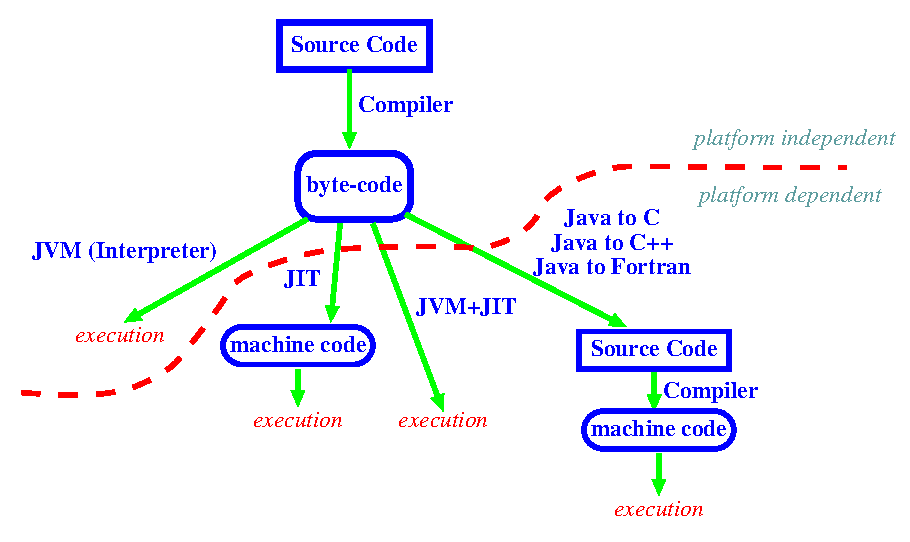
\includegraphics[width=\textwidth]{../Figures/Java_Overview.eps}
    \caption{Overview of the Java language execution model.}
    \label{fig:Java_Overview}
  \end{center}
\end{figure}

So for every platform, where a virtual machine is available,
you can execute the byte-code without any compatibility problems.
But the ``look and feel'' can be different: for example Java buttons
in Windows look different from buttons in X11/Motif using a UNIX
operating system. But if you use the new Swing components supplied
with the Java 2 standard or extend the Java 1.1 standard with the Swing
components, you can choose the appearance of the graphical look, which then
is the same across all platforms. So if you are using the new Java 2 standard
(JDK1.2), you should definitely use the new Swing components. If you
still use the AWT components (like we do here in this book), you should
keep in mind that the look (not the functionality) 
of the program can be different on different platforms. 
A big advantage of the Swing components is that they do not use any
native code, which the AWT components do.

The main reason for the wide availability of Java
is that SUN Microsystems distributes the Java Development Kit (JDK)
freely for a number of important platforms (Windows, Solaris/Linux,
other Unix systems). The JDK consists of a compiler (javac), a
debugger (jdb) and a virtual machine (java)\footnote{Actually, there
are some more components like the javadoc command to create HTML
documentation or the jar tool to create zipped packages of
class files belonging together - see Chapter \ref{sec:javadoc}}.

The JDK can be downloaded from the Internet from the 
\href{http://www.javasoft.com}{JDK Javasoft link page}.
The latest version, as of the time of writing, is 1.2. 
Throughout the book,
we will use the Java 1.1 language version and the JDK 1.1.7,
because the Java 2 standard is not yet implemented in any JVM of the
web browsers available.

The only additional thing necessary to have a Java programming
environment is a text-editor to write the Java programs.
Use your favorite editor, e.g. emacs or xemacs, which are
also freely available and have nice Java editing modes.

There is also a freely available IDE (Integrated Development 
Environment) called \href{http://www.freebuilder.org/}{FreeBuilder}.
This is a complete environment to write Java programs comfortably.
Since it is the first running under the GNU license, it is free, but
still in alpha development stage, but it already comprises a lot of features. Of
course, there are many commercial IDEs available, like SUN's Java Workshop
or Simplicity for Java.


Opposing to other languages, which use the ASCII character set, Java
uses the  \href{http://unicode.org}{Unicode character set}.
Unicode consists of characters represented
by 2 bytes instead of 1 byte like in the ASCII set. So you can use 
all the 38885 different
characters available in the Unicode set (Version 2) for writing a Java program.
This means you can name your variables using for example Japanese or Greek
characters. Right from the beginning, Java is an international language.

Java is also case sensitive and doesn't need any special characters
to mark continuation lines as is necessary in Fortran for example.

Comments are used just like in C and C++.
You can use either the /* \ldots */ syntax (borrowed from C) for
multi-line comments or the // syntax (borrowed from C++) for single
line comments. Additionally you can use /** \ldots */ for comments
to automatically generate a HTML documentation file for the class
defined in the file. We will see in Chapter \ref{sec:javadoc} 
how this can be achieved.
 
There are also certain disadvantages, which should not be forgotten
to mention: The learning curve is certainly steeper for the beginner
for Java than for Matlab or even Fortran. This is of course due
to the full use of the object oriented approach used for all Java
programs. This clearly shows up when we will introduce e.g. the
file and keyboard input/output capabilities of Java.
But in the long term, learning Java definitely pays off. 

A second point to note is, that for scientists a big concern are always
complex numbers. They are currently not supported as primitive types as 
in Fortran for example, but there are (standardized) packages, which
add complex number support to Java (e.g. JNL). And the CJ compiler,
an extension to the Java compiler, can even handle primitive complex types.


\subsection{The ``HelloWorld'' Program -- Applications and Applets}
\label{sec:HelloWorld}

\subsubsection{Application}

Now let us start with the traditional ``Hello World'' program written
in Java. Type the following code using your favourite text editor 
and save the program in a file called \verb|HelloWorld_Application.java|.
\inputlisting{../Listings_Java/HelloWorld_Application.java}

If we use the JDK 1.1 or 1.2 under Windows or Unix, we can execute
the above example by typing on the command line:
\begin{itemize}
\item Compiler: \verb/javac HelloWorld_Application.java/  \\
  $\Longrightarrow$ produces HelloWorld\_Application.class 
  in the same directory.
\item Byte-Code Executor (JVM):  \verb/java HelloWorld_Application/
\item Output on screen: \verb|Hello World !|
\end{itemize}
Let us now try to understand the above code. The program consists of
three lines. 

In the first line the program declares 
with the help of the \texttt{class} statement a class called 
\verb|HelloWorld_Application|. 
The identifier following the \texttt{class} statement is
the name by which the class will be referenced. Each Java program
is a class. The definition of the class is included in the curly brackets
between line 6 and line 10.

In the second line the \verb|main| method is introduced. The main
method is declared \verb|void| because the method does not return a
value. The main method is executed when you run the class as an
application. The only parameter, the argument
of the main method, is an array of String objects, here named \verb|args|.

In the third line the method \verb|println()| of the system class 
\verb|out|
is invoked. This method simply prints a string and terminates with a 
new--line command. Alternatively you could use the 
\verb|System.out.print()| method, which does the same, but does
not print a newline at the end. 

You have just written and executed your first application in
Java. Please, do not worry if you do not understand everything. You are
not expected to understand everything at this stage.

If you are using Emacs/Xemacs and JDE you could have started Emacs and
then just used the ``JDE New'' method in the ``Files'' menu. Then you
have to type the \verb|System.out.println()| code, which could
again be accomplished by using the \verb|Generate| menu in the
JDE menu. To compile
use the ``compile'' command in the ``JDE'' menu and similar
the ``run'' command in the same menu.  

\subsubsection{Applet}
\label{sec:Applet}

Java offers another possibility to execute programs, the so-called Applets.
In contrast to the stand--alone Java application which starts with a
\verb!main! method and runs until it is completed, the applet is a kind of
sub--program which runs under the control of some other program.
Usually, applets are (small) Java programs, which are started by a 
server program,
e.g. a WWW browser like Netscape Navigator\footnote{You need at least 
version 4.06 or patches for earlier versions to use all features of Java 1.1}, 
the Internet Explorer\footnote{Seems to run Java 1.1 programs since
version 4, but does not conform to the Java standards.},
HotJava or the appletviewer\footnote{included with the JDK.}.

In the case of an applet, you have a browser loading a HTML 
(Hyper Text Mark-up Language) file. This HTML file contains
mark-ups, which tell the browser what applet to load and
where to find the applet (see figure \ref{fig:HTMLOverview}). 
\begin{figure}[htbp]
  \begin{center}
    \includegraphics[width=\textwidth]{../Figures/HTMLOverview.eps}
    \caption{An HTML file gets loaded into the browser. The browser itself formats the text and if it finds an applet mark, it starts the applet.}
    \label{fig:HTMLOverview}
  \end{center}
\end{figure}
You should note that HTML is not a programming language, but
it is a mark-up language to produce a text with additional
``commands'' for the meaning of the text parts. It does
not give any details about the formatting or layout of the
text. To start an applet, HTML uses some special marks, which we
will discuss in a moment.  

The big difference between an applet and an application is that
applets are not allowed to do certain things. For example applets
do not have access to local file systems, so it is not possible
to save data on the file system from an applet. It is also not
possible for an applet to issue a print command, the process of
printing has to be initiated by the server (browser). 
And an applet is not allowed to do time consuming tasks like
long computations. This has to be kept in mind, when writing
applets.


The ``Hello World'' example written as an applet takes the following form:
\inputlisting{../Listings_Java/HelloWorld_Applet.java}

Applets have to be derived from the applet class
\verb|java.applet.Applet|, which include the principal facilities of
the Abstract Windowing Toolkit (AWT) and the interface with X/Motif on
Unix, Windows on PC, and Mac-OS on Macintosh platforms.
As you can see there is no main method in an applet. Instead if an applet
is started by a server, the init() method is executed first. There is also
a start() and a stop() method, which are executed if the applet becomes
visible or disappears in the server window (e.g. by scrolling in the
Netscape Navigator window).

Many methods are available to set up the display in an assigned applet area.
The paint() method appearing in the ``Hello World'' applet is
responsible for the visual part of the applet. It uses a canvas
(drawing area) with a size defined by the calling HTML file. In our case
this HTML file could look like:
%% Listings V0.20 ERROR ?????
%%\lstinputlisting[language=HTML]{../Listings_Java/call_HelloWorld_Applet.html}
\lstinputlisting{../Listings_Java/call_HelloWorld_Applet.html}
The code parameter given in the HTML file defines the name of the applet
to be executed. Because there is no init() and no start() method in our
example, the paint() method is called by the browser or appletviewer.
The size of the canvas has to be given explicitly in pixels in the
HTML file.

To run the applet you can either type
\begin{itemize}
\item \verb|appletviewer  call_HelloWorld_Applet.html| or
\item use the following URL in the browser: \\
        \verb|PATH_TO_CLASS_AND_HTML_FILE/call_HelloWorld_Applet.html| \\
        e.g. \verb|/home/user/java/call_HelloWorld_Applet.html|
\end{itemize}

The question, when to use an application and when to use
an applet, is difficult to answer. We have decided to write most
of the programs as applications and applets in one program. So you
can decide if you run it as an application or start it as an applet.
Some features are of course not available from an applet and
you are missing some functionality of some programs, if you run them
as an applet.
Time consuming calculations should
definitely be written as an application, small programs can be
written as an applet. Although this is not mandatory it should
be obeyed by a good Java programmer.

In Java 1.1 a new package has been introduced, which allows for
so-called ``trusted applets''. These are specially signed libraries,
which are signed with a key by a person we trust 
(using the JDK we have to use \verb|javakey| for that purpose). Only if the
signature is valid and we trust that person, the ``trusted applet''
has access to the local files system -- basically it can do everything
an application could do on our machine (see \cite[page 142]{javanutshell}).
 This is already implemented with
the appletviewer, on other ``servers'' it might work or not. In the
future this will be extended to a more extensive set of rules for the
allowed methods of an applet.

\paragraph{Documenting Java Programs -- javadoc}
\label{sec:javadoc}
A last remark concerns the documentation for the programs. We have
learned, that we can include documentation comments using 
\verb|/** .... */|. These comments are processed by using the
\verb|javadoc| command from the JDK. If you run the javadoc command as: 
\begin{sverbatim}
  javadoc HelloWorld_Application.java HelloWorld_Applet.java  
\end{sverbatim}
you get some HTML files: packages.html, tree.html, AllNames.html,
HelloWorld\_Applet.html, HelloWorld\_Application.html. All these
files describe the written classes. The tree.html file gives a tree
showing the relatives of the class. The package.html gives the
package structure (not used here). The most important file is the
AllNames.html, which is an index of all written programs in this package
(for an introduction to packages see later).

You can even include special predefined strings to supply the
author and many more informations to the javadoc command, either
for a class or a method, whereas the documentations for the method
can also be supplied for a class:
\begin{lstlisting}{}
  /**
      @author Peter Biechele
      @version 1.0
  */
  .. class ... { }

  /** 
      @see <a class name>
      @see <class name>#<method name>

      @param  a b c
      @return d
      @exception  none
  */
  .. method ... { }
\end{lstlisting}

This of course gives us the opportunity to write our 
explanations/documentation
between the \verb|/** .... */| commands using HTML constructs like
\verb|<hr>| for a horizontal rule or others - try it. 
Because this code gets directly included in the HTML files produced by
the \verb|javadoc| command, you can have nicely formatted documentation.
But you should avoid using \verb|<h1>| to \verb|<h6>| -- the heading 
commands -- because javadoc uses them for its own structure.

If you load AllNames.html into a browser, you get the HTML file shown
in figure \ref{fig:javadoc1}.
\begin{figure}[htbp]
  \begin{center}
    \leavevmode
 \includegraphics[width=8cm]{../Figures/AllNames.eps} 
    \caption{The output of the \texttt{javadoc} command from the JDK 1.1.}
    \label{fig:javadoc1}
  \end{center}
\end{figure}
Now you can click on the link HelloWorld\_Applet and you get the
documentation for that class and analogous for the HelloWorld\_Application
class (see figure \ref{fig:javadoc2}).
\begin{figure}[htbp]
  \begin{center}
    \leavevmode
  \includegraphics[width=6cm]{../Figures/HelloWorld_Applet.eps}
  \includegraphics[width=6cm]{../Figures/HelloWorld_Application.eps}
    \caption{The output of the \texttt{javadoc} command from the JDK 1.1.}
    \label{fig:javadoc2}
  \end{center}
\end{figure}
The missing graphics on the right of figure \ref{fig:javadoc2} 
are available in the Java documentation of the
JDK and just has to be copied into a subdirectory  
of the HTML directory called \verb|images| . 
Then it looks like the figure on the left.

The javadoc command of the JDK 1.2 produces much nicer pages which
look like in figure \ref{fig:Java2HTMLDoc}. There are no separate 
gif pictures
needed anymore and the structure of the classes is represented
much better.
\begin{figure}[htbp]
  \begin{center}
    \subfigure{\includegraphics[width=.3\textwidth]{../Figures/HelloWorldApplet1.eps}}
\quad \subfigure{\includegraphics[width=.3\textwidth]{../Figures/HelloWorldApplet2.eps}}
\quad \subfigure{
\includegraphics[width=.3\textwidth]{../Figures/HelloWorldApplet3.eps}}
    \subfigure{\includegraphics[width=.45\textwidth]{../Figures/HelloWorldApplication1.eps}}
\quad \subfigure{
\includegraphics[width=.45\textwidth]{../Figures/HelloWorldApplication2.eps}}
    \caption{The output of the \texttt{javadoc} command from the JDK 1.2.}
    \label{fig:Java2HTMLDoc}
  \end{center}
\end{figure}

%%%%%%%%%%%%%%%%%%%%%%%%%%%%%%%%%%%%%%%%%%%%%%%%%%%%%%%%
\subsection{Variables}
\label{sec:Variables}

Essentially, Java distinguishes between two types of variables,
primitive data types and reference data types.
\subsubsection{Primitive data types}
\label{sec:primitive_data_types}
We already mentioned that in Java each variable or expression has a
definite type and that each type has identical size and behaviour on
all Java implementations.  Java has built in primitive data types
to support integer, floating--point, boolean, and character values.
The primitive data types of Java for integers, floating--points,
characters and boolean variables are listed in Table
\ref{table:primitivedata}.
\begin{table}[htbp]
\label{table:primitivedata}
\begin{center}
\begin{tabular}{l|l|l|l|l}
Type & Contains & Default & Size & Min \\
     &          &         &      & Max \\ \hline \hline
byte  & signed integer & 0 & 8bits & -128  \\
&&& & 127    \\ \hline
short & signed integer & 0 & 16 bit &-32768 \\
&&& & 32767 \\ \hline
int &   signed integer & 0 & 32 bits&-2147483648 \\
&&& &2147483647 \\ \hline
long & signed integer & 0 & 64 bits &-9223372036854775808\\
&&& &9223372036854775807\\ \hline
float & floating--point & 0.0 & 32 bits &$\pm$1.40239846E-45\\
&&& &$\pm$3.40282347E+38\\ \hline
double & floating--point & 0.0 & 64 bits &$\pm$4.94065645841246544E-324\\
&&& &$\pm$1.79769313486231570E+308\\ \hline
boolean & true or false      &  false & 1 bit&\\
&&&       &  \\ \hline
char  & Unicode character & $\backslash$u0000 & 16 bits & $\backslash$u0000 \\
&&& &$\backslash$uFFFF   \\ \hline
\end{tabular}
\end{center}
\caption{Primitive data types in Java. The byte and char data types have
  been introduced in Java 1.1 and in Java 2 there was a void type added.}
\end{table}


The following comments have to be made. In a Java program every
variable must have a type that precedes its name when the variable is
declared. For example the integer i may be declared as
\begin{sverbatim}
int i;
\end{sverbatim}
and integer or long values can be expressed as
\begin{sverbatim}
int i = 123; 
long l = 1234567889L;     long l2 = 123456789l;
\end{sverbatim}

Characters are represented by two different data types in Java.
One can store only one character and is called char. The other
one stores many characters like a word or even a sentence. This
second datatype is not a primitive datatype but an object and is
called string. It will be discussed later on.

Char values are defined in Java between single quotes, e.g.
\begin{sverbatim}
char c = 'C';
\end{sverbatim}
Usually characters on a computer are represented internally by a number.
This number is between 0 and 255 and the coding of the characters
to the numbers is called ASCII\footnote{American Standard Code 
for Information Interchange} code. Because not all characters used
for all the different languages in the world are representable by
256 different codes, the codespace has been extended to 65535
numbers and is now called Unicode character set. With this set of
numbers corresponding to characters you can code every language
of the european countries. There are other Unicode sets to represent
more complicated languages like Japanese or Chinese.

A Unicode character in Java is represented by the Unicode escape sequence
$\backslash$uxxxx, where xxxx is a sequence of four hexadecimal digits.

Float and double types have special values that may be the result of
certain floating-point operations. For example in the java.lang.Float
and java.lang.Double classes the special values
\verb|POSITIVE_INFINITY|, \verb|NEGATIVE_INFINITY|, and 
\verb|NaN| (not-a-number) are
defined.

Floating point numbers are expressed as e.g.
\begin{sverbatim}
13.       1.3e1        .13E2 
\end{sverbatim}
and are considered to be constants of type \verb|double| 
unless they are specified with \verb|f| or \verb|F|, which makes them
then \verb|float| constants.

In Java strings are not of primitive type and they are not an
array of chars like in C. Java provides a String
class to deal with sequences of character data. The java string
class provides methods to operate on String objects.

All variables in Java are initialized automatically, as soon as they
are declared. All primitive types get initialized to zero, the boolean type
to false and all objects (remember they are references) are initialized
to \verb|null|. So there is no ambiguity like in other languages, if
a variable has a defined value at certain points of the program. 
Although Java forces you to include sometimes a statement to
initialize variables, just to make easier to read source code.
We will see an example for this later on, when we discuss loops
and calculate averages of sequences of numbers.

\subsubsection{Reference data types}
\label{sec:Reference_data_types}

All non-primitive data types in Java are objects. They are
called also ``reference types'' because they are handled by
reference. For example you may pass the address of an object, which is
stored in a variable, to a method. In contrast, primitive types are
always passed by value.

\subsubsection{Strings and Arrays}
There are two special data types belonging to the reference data types:
the arrays and the strings. Arrays are objects, which have some
special properties and are handled a little bit different from
ordinary objects, just because they are used very often (see section
\ref{sec:Arrays}).

Strings are another special data type belonging to the reference data 
type. In contrast to C and C++ they are not arrays of char variables,
but seperate objects, which can only be accessed as the whole string or
by using special string functions. The strings are also not terminated
by a \verb|\0| like in C/C++, they just contain the text string
assigned to the string object. In the section about arrays, we will learn
how to handle Strings and in the section about objects, we will finally
hear the full story. Actually we hav met strings in out first program
already, because the text between two \verb|"| is a string.


%%%%%%%%%%%%%%%%%%%%%%%%%%%%%%%%%%%%%%%%%%%%
\subsection{Casting and Type Conversions (Wrapper Classes)}

Java uses a clear strategy to convert the primitive data types to 
other primitive ones. In a calculation Java always converts (casts)
the less precise type to a more precise one. So if you multiply an
integer and a float value, it converts automatically the integer to
a float and then multiplies both values. If you want to convert
a value explicitly you can use the cast operators (like in C and C++).
Just write the primitive type in round brackets in front of the value to
be converted, e.g. \verb|result=(double)a*b| casts \verb|a| to 
a double value and
then multiplies it with \verb|b|, assigning the result to \verb|result|.
You can also use the wrapper classes to be discussed below, but
it is much more complex and should be avoided.

A common problem is to convert from strings to primitive types and
vice versa. Because strings are objects and not primitive types, we
need a method for the conversion. For that reason Java has so called
wrapper classes, subclasses of the \verb|java.lang.Number| class 
for all primitive data types. 
These classes provide all the necessary methods for all types of
conversion. 

The static \verb|.valueOf(String s)| method always converts a string
to the corresponding wrapper class of a primitive type, e.g. 
\begin{lstlisting}{}
        double a;
        String text="+1.234";

        Double D = Double.valueOf(text);
        a = D.doubleValue();

        a=Double.valueOf(text).doubleValue();
\end{lstlisting}
The fourth line converts the string to the \verb|Double| class and in the
fifth line 
the \verb|doubleValue()| method converts the Double wrapper class 
to a double primitive type. The last line shows how to do it in
one line.
For the other types you just have to substitute float or int 
for double, i.e., \verb|floatValue()|, \verb|intValue()| and the
corresponding wrapper class (\verb|Integer| for \verb|Double|, etc.).
 
Another (easier) method, 
later used in the \verb|ParamApplet.java| program is, e.g.,
the \verb|Integer.parseInt(String s)| method, which gives back a primitive
type integer instead of the wrapper class like \verb|valueOf(String s)|.
For other conversions you can use the \verb|Long.parseLong(String s)| or the
\verb|Long.parseByte(String s)| method.

These methods  simplify the conversion a little bit. For the example, see
\verb|ParamApplet.java| in line 11. But this method is only 
available to Integer, Long and Byte wrapper classes, NOT for
Float and Double as of Java 1.1. Fortunately they are included in the
Java 2 specification.
In the Java 1.1 case you have to use the \verb|valueOf(String s)| and
\verb|doubleValue(String s)|, \verb|floatValue(String s)| methods.

To convert a double value to a string you have to use the 
\verb|toString(double d)|
method, which is available for all primitive data types.
For example, two ways of doing it are:
\begin{lstlisting}{}
  double d = 3.1234;
  String s1 = Double.toString(d);    <------ most easy way
  String s2 = (new Double(d)).toString();
\end{lstlisting} 

\paragraph{Convenience Classes of the simulation Package for Conversions}
The \verb|simulation| package provides in the \verb|util| class methods
to convert all primitive types to Strings and Strings to primitive types.
Therefore we can for example use 
\begin{sverbatim}
  double dum = simulation.Util.stringToDouble("23.4567");
  String text = simulation.Util.doubleToString(7.4562);
\end{sverbatim}
to convert a String to a double or a double to a String. There are analogous
methods to convert int, long and float variables. 

%%%%%%%%%%%%%%%%%%%%%%%%%%%%%%%%%%%%%%%%%%
\section{Packages and Import Statements}
\subsection{Packages}
\index{packages}
Because Java was designed to be able to load code distributed
over the whole internet dynamically, you have to avoid name conflicts
between the programs/classes. The Java solution 
for an Internet--wide unique naming scheme is to put
every class in a \emph{package}. A package  is a group of related
and possibly cooperating classes. The naming scheme should be based on the
internet domain name of the organization at which the package is developed.

If we are not using the package command at all, Java uses the \emph{empty 
package}. \index{empty package}
Then we have to put our programs into the current directory.
This is not recommended for medium to complex programs, but for
test purposes and very small programs this is very convenient.

\index{import statement}
The name of the package is given
at the beginning of a file before the actual program/class
definition starts. So for example if we put the statement
\begin{quotation}
  \verb/ package de.freiburg.simulation; / 
\end{quotation}
at the beginning of the ``Hello World'' application, we can compile
the application with \verb/javac HelloWorld_Application.java / like before.
But to run the application we have to use
\begin{quotation}
  \verb/ java de.freiburg.simulation.HelloWorld_Application / . 
\end{quotation}
The program does not start? It cannot, because
there is one more thing to know. Java is looking for programs/classes
in the directory structure given by the package and the class name. So
for the example above we have to put the 
\verb/HelloWorld_Application.class/ file
in the directory \verb|de/freiburg/simulation/| and issue the \verb|java|
command in the directory, where the directory tree starts.

For example on a Unix machine execute:
\begin{sverbatim}
 mkdir de
 mkdir de/freiburg
 mkdir de/freiburg/simulation
 cp HelloWorld_Application.class de/freiburg/simulation/
 java de.freiburg.simulation.HelloWorld_Application
\end{sverbatim}
On a Windows machine we have to change the \verb|mkdir| command into
the \verb|md| command and \verb|cp| into \verb|copy|.

\index{classpath}
\index{CLASSPATH}
We can also use an environment variable called \verb|CLASSPATH| to tell
the java executor (JVM) where to find the class files. 
If for example the
\verb|CLASSPATH|-variable includes the directory \verb|/home/user/java|
you can
start the above example in this directory, if the class is in the 
subdirectory  \verb|de/freiburg/simulation/|. It has to be noted that
the entries in a \verb|CLASSPATH| specification may also be ZIP files
that contain these classes. On Unix systems the directories in a
\verb|CLASSPATH| specification are separated by `` :'' ( on Windows systems
by ``;'').

For example on a Unix system:
\begin{sverbatim}
 export CLASSPATH="$CLASSPATH:/home/user/java"
 cd /home/user
 java HelloWorld_Application
 java de.freiburg.simulation.HelloWorld_Application
\end{sverbatim}
Only one of the last two lines have to be used, depending on the
location of the class file. On Windows you have to change the first
two lines to
\begin{sverbatim}
  set CLASSPATH="%CLASSPATH;c:\java"
  cd c:\
\end{sverbatim}

All the standard API classes of Java are stored in a central jar
file, which is additionally packed to save disk space. These classes
are always searched, no matter the \verb|CLASSPATH|-variable is set to.
This might be different on some systems and the Java API class file
path has to be included in the \verb|CLASSPATH|-variable. 


\subsection{The jar Tool}
If you have written a lot of small classes, which all work together
(called a project), you
can put them all inside a ``jar'' file and give the jar file
to friends instead of the whole bunch of small class files.
A jar file is just an archive created by the \verb|jar| program 
coming with the JDK. It works like the well-known UNIX \verb|tar|
command. This is actually a very nice method for packaging
applets on the internet, because the jar command also compresses
its contents. 

For example to view the contents of a jar file you can issue the command
\verb|jar tvf lava.jar|. The file \verb|lava.jar| is a file on the
CD ROM of the Lava Rocks package. You can use any other \verb|.jar| file
you have or can find anywhere. Some of the
available options used with jar are given in table \ref{tab:JarOptions}.
\begin{table}[htbp]
  \begin{center}
    \begin{tabular}{cp{0.7\textwidth}}
      Option & Description \\\hline
      c & create jar file\\
      t & table of contents of jar file\\
      x & extract files from jar archive\\
      f & name of jar file comes as first argument after options (the
          default is the standard input/output) \\
      v & verbose output \\
      O & do not compress (used for jars residing in the CLASSPATH)\\
    \end{tabular}
    \caption{Options of the jar command. The jar tool is included in the JDK.}
    \label{tab:JarOptions}
  \end{center}
\end{table}
Jar files are portable from one platform to the other, but as you can 
see jar is not as powerful as the tar command in UNIX.

\subsection{Basic Java Organization}
Java is basically defined in two ways: the first one is the basic
set of instructions, like all variables, all arithmetics and conditional
statements and loops (see in the next few sections). This is the
fundamental part of the language. 

The second one are the Application Programmers Interfaces (API).
They are just packages, which consist of many functions and variables
to provide a certain functionality. For example the applet API (package)
provides all the necessary functions to build and handle applets
in Java. 

The big difference to other languages like C for example, where also
certain (small) APIs exist, is that these APIs are all included
in the Java standard, including the ones giving access to graphical
capabilities. There is no place for different vendors to supply
different libraries (packages) for the same functionality, but
using different calling schemes and therefore making programs
non portable. 

\subsection{Import statement}
Before learning more about the syntax of Java, we have to explain another
statement appearing in the part of any Java program before the actual
definition of the class: the \verb|import|-statement. With \verb|import|
you can make classes available, so you don't have to use the fully
qualified name to the class, which would be very long sometimes. 

If you would like to
use the HelloWorld class from above in your programs, you have to change
the \verb|main()| method to let us say \verb|hello()|. 
\loadlisting{HelloWorld.java}{../Listings_Java/HelloWorld.java}
Now you could either
type \verb|de.freiburg.simulation.HelloWorld.hello()| (the fully qualified 
name) in your program or you can use
\begin{sverbatim}
import de.freiburg.simulation.*;
....
   HelloWorld.hello();
\end{sverbatim}
to import all classes in the \verb|de.freiburg.simulation| class.
You can also use:
\begin{sverbatim}
import de.freiburg.simulation.HelloWorld;
....
   HelloWorld.hello();
\end{sverbatim}
if you just want to import one special class. But you can not use 
\verb|import de.freiburg.*;| and then call the method by using
\verb|simulation.HelloWorld.hello();|. You can not split the
package name in the import statement.

We have already made use of the \verb|import|-statement in the ``Hello World'' 
applet. There we have imported the \verb|java.applet|-class, which
defines applets and their behaviour, and the \verb|java.awt|-class, which
will be explained later.
 
There is one class, which is always imported without any import statement:
the \verb|java.lang.*| classes. This is the fundamental class of Java and it is
implicitly imported for all Java programs, so you do not have to specify
it. For example the System class is in \verb|java.lang|, that is why
we did not have to use an import statement in the ``Hello World''
application.  

%%%%%%%%%%%%%%%%%%%%%%%%%%
\subsection{Compiling Projects}
If you write a program consisting of many classes and files, you
may think that this is a lot of work to compile all of them. Or if
you are used to writing code in other languages, you might think
of using tools for checking if a program has to be recompiled, if you make
changes to some files. One of these tools might be the famous ``make''
utility. But fortunately this is not needed for Java, because
the JDK developers (or to be precise the Java standard) already
takes care of these problems. 

You have to arrange your code in the different classes according to 
certain rules (packages). So the directory structure is already a
nice tree structure of your project. 

If you then want to compile
the whole project, but only the files which have changed\footnote{Notice
that there is no dependence of classes on other classes in the
sense of re-compilation. Java does dynamical run-time linking and no static 
linking at the end of the compilation process as in all other languages.}
should be recompiled, you issue the
command 
\begin{sverbatim}
javac -depend -d base_directory main.java
\end{sverbatim}
then the Java compiler takes care of all ``dependencies''.   

%%%%%%%%%%%%%%%%%%%%%%%%%%%%%%%%%%%%%%%%%%
\section{Simple Arithmetics, Conditional Statements and Loops}
\label{sec:Loops}

\subsection{Simple arithmetics}
As we already mentioned Java  supports almost all of the standard
C operators. The arithmetic operators that operate on numerical types
are 
\begin{center}
\begin{tabular}{ll}
$+$ & addition \\
$-$ & subtraction                 \\
$*$ & multiplication \\
$/$ & division \\
\% & remainder
\end{tabular}
\end{center}
The $+$ operator can also be used to concatenate strings, as we will
see later in an example in section \ref{sec:Parameter}.

It is important to remark, that in Java integer division truncates
toward zero (7/2=3, -7/2=-3 and -7/-2=3).

Java has two special operators for increment $++$ and decrement $--$. The 
expression \verb|i++| is equivalent to \verb|i=i+1| except that
\verb|i| is evaluated only once. They can be used as pre- and post-operators,
depending on the position of the symbols, e.g. \verb|i++| or \verb|++i|.
This does not make a difference, if you just have these statements
alone, but in some complex expressions this might make a difference.
The postfix (prefix) version of the operator ++ evaluates  the value
of the operand before (after) the increment operation.
For example \verb|i = j++| means setting i to j and then increment j by one.
But \verb|i = ++j| means setting i to j+1.

There is no power operator like \verb|**| in FORTRAN or \verb|^| like in many
different programs like TeX/LaTeX. In Java like in C/C++ you have to use
(like in C) the \verb|Math.pow()| method of the \verb|Math| class.
The \verb|^| operator, used sometimes for the power, is the exclusive
or (XOR) operation in Java (either in the logical or the boolean sense). 
We should not confuse this. 

Java supports also a standard set of relational and logical operators,
which all yield boolean values. They are listed below

\begin{center}
\begin{tabular}{ll}
$>$  & greater than \\
$>=$ & greater than or equal to \\
$<$  & less then \\
$<=$ & less than or equal to \\
$==$ & equal to \\
$!=$ & not equal to
\end{tabular}
\end{center}


The conditional operators
\begin{center}
\begin{tabular}{ll}
\& \& & conditional AND      \\
$\mid\mid$ & conditional OR
\end{tabular}
\end{center}
operate on  boolean expressions only.

Java has also bitwise operators which operate on integers and on
boolean types. They allow to perform bit manipulation on data.
\begin{center}
\begin{tabular}{lp{0.8\textwidth}}
\& & and \\
$\mid$ & or \\
$\tilde{}$ & not \\
$<<$ &  shifts bits left filling with zero bits on the right \\
$>>$ & shifts bits right filling with the highest sign bit on the
           left--hand side (like a division by 2)\\
$ >>>$ & shifts bits right filling with zero bits on the left--hand side, treating
    the argument as a bitfield
\end{tabular}
\end{center}
Some examples are in place
\begin{sverbatim}
 1 & 0   // is zero
 1 | 0   // is one
 ~10     // is -11, do it by hand to check
 2 << 1   // is 4, because bitwise is 2=0010 and 4=0100
 2 >> 1   // is 1, because bitwise is 2=0010 and 1=0001
 2 >>> 1  // is also 1, like above
 2 >> 3   // is 0, because bitwise is 2=0010 and 1=0000
\end{sverbatim}
You can use these operators for doing fast divisions by powers by $2$, 
because it is much
faster to do a bitshift than a division. For example, instead of
writing \verb|16/2| use \verb|16 >> 1| or instead of using \verb|8/4|
we can write \verb|8 >> 2|. 

Last not least we have to mention the fundamental assignment operator
$=$. It may be used in combination with other operators, e.g., $+=$
means is incremented by.


\subsection{Loops}
\paragraph{for Loops}
For our forthcoming applications the most important control statement
is the \verb|for| statement. It is used to loop over a range of values
from the beginning to the end. Its syntax is
\begin{sverbatim}
for (init_expressions; boolean_expr; incr_expressions) {
    statements
}
\end{sverbatim}
where \verb|init_expressions| denotes the initial value of the iterated
variable, \verb|incr_expressions| denotes the increment of the iterated
variable. For both you can specify more than one expression separated
by commas (as in C). This is the only place, where you can use these comma
separated lists. The variables used in the for statement can be 
integer (long) or float (double) values. 

At the beginning of the \verb|for| loop the boolean expression
\verb|boolean_expr| is evaluated. If its value is found to be 
\verb|true| the statement is executed repeatedly with increment
\verb|incr_expr| until the value of the boolean expression is found to
be \verb|false|.

As an example demonstrating the use of
\verb|for| loops we want to write a program to calculate the mean of
a given number of random numbers. One possible implementation
could look like this:
\inputlisting{../Listings_Java/DataMean.java}

Here we used the class \verb|java.util.Random| which allows for
the creation of random numbers. If we don't supply a seed, as is the
case here, it just uses the time to initialize the generator. The
initialization takes place in line 10, where a new generator is created.
You can check this by running the application more than once and comparing
the means -- they should not be the same. 

The \verb|next.Double()| method returns a new random number of type
double (for a float use \verb|rand.nextFloat()|). You can also create normally 
distributed random numbers with the \verb|nextGaussian()| method of
the \verb|Random| class.
The remaining parts of the program should be self explaining. You can of
course use any expression (e.g. \verb|d=d*u+2|) 
in the last part of the for statement, not only
the \verb|++| operator, which is obviously used most often. 

\paragraph{Byte-Code of a class file}
Using the \verb|DataMean()| program, we want to show the byte-code
produced by the Java compiler. In the first line you can see the
command to use (\verb|javap|) and below the output:
\begin{scriptsize}
\begin{verbatim}
Command_Line>>> javap -c DataMean

Compiled from DataMean.java
public synchronized class DataMean extends java.lang.Object
    /* ACC_SUPER bit set */
{
    public static void main(java.lang.String[]);
    public DataMean();
}

Method void main(java.lang.String[])
   0 sipush 10000
   3 istore_3
   4 new #10 <Class java.util.Random>
   7 dup
   8 invokespecial #12 <Method java.util.Random()>
  11 astore_1
  12 dconst_0
  13 dstore 4
  15 iconst_1
  16 istore_2
  17 goto 32
  20 dload 4
  22 aload_1
  23 invokevirtual #17 <Method double nextDouble()>
  26 dadd
  27 dstore 4
  29 iinc 2 1
  32 iload_2
  33 iload_3
  34 if_icmplt 20
  37 dload 4
  39 iload_3
  40 i2d      
  41 ddiv
  42 dstore 4
  44 getstatic #18 <Field java.io.PrintStream out>
  47 new #8 <Class java.lang.StringBuffer>
  50 dup
  51 ldc #2 <String " The mean of ">
  53 invokespecial #13 <Method java.lang.StringBuffer(java.lang.String)>
  56 iload_3
  57 invokevirtual #15 <Method java.lang.StringBuffer append(int)>
  60 ldc #4 <String " random numbers
">
  62 invokevirtual #16 <Method java.lang.StringBuffer append(java.lang.String)>
  65 ldc #3 <String " between 0 and 1 is ">
  67 invokevirtual #16 <Method java.lang.StringBuffer append(java.lang.String)>
  70 dload 4
  72 invokevirtual #14 <Method java.lang.StringBuffer append(double)>
  75 ldc #1 <String " !">
  77 invokevirtual #16 <Method java.lang.StringBuffer append(java.lang.String)>
  80 invokevirtual #20 <Method java.lang.String toString()>
  83 invokevirtual #19 <Method void println(java.lang.String)>
  86 return

Method DataMean()
   0 aload_0
   1 invokespecial #11 <Method java.lang.Object()>
   4 return
\end{verbatim}
\end{scriptsize}

\paragraph{while and do--while}
Java offers also the possibility to use other loop constructs, the
\verb|while| and the \verb|do-while| loop. There syntax is
\begin{sverbatim}
while (boolean_expression)
 statement
\end{sverbatim}
and
\begin{sverbatim}
do
  statement
while (boolean_expression)
\end{sverbatim}
It is important to observe that in the first construct the boolean
expression is evaluated \textit{before} the statement is executed, while in
the second construct the boolean expression is evaluated \textit{after} the
statement has been performed!

In order to give an example we write down an equivalent code using
the
\verb|while| statement of the \verb|for| loop of the
\verb|DataMean.java| program. Lines 13 to 15 have to be replaced by
\begin{sverbatim}
int i;
while(i<N){
  mean += rand.nextDouble();
  i++;
}
\end{sverbatim}

\subsection{Conditional Statements}
\paragraph{if-else}
The \verb|if| statement is the fundamental form of conditional control
of flow. It allows to choose, whether the statements that follow it are
executed or not. Its syntax in Java is
\begin{sverbatim}
if (boolean_expression) {
   statement1
}
else if (boolean_expression) {
   statement2
}
else {
   statement3
}
\end{sverbatim}
First, the boolean expression is executed. If the value is \verb|true|
then \verb|statement1| is performed, otherwise if there is the
optional \verb|else| statement \verb|statement2| is executed. Of
course, \verb|if-else| constructions can be nested, i.e., an
\verb|if-else| conditional control flow, can be placed within another
\verb|if-else| statement.

\paragraph{The conditional operator ?} The conditional operator ?
provides a single expression yielding one of two alternatives depending on
a boolean expression. To demonstrate its use we write down an
\verb|if/else| Java code first and translate it into an equivalent  ? 
construction. The \verb|if/else| code reads

\begin{sverbatim}
if (a<b) 
  x=1.0;
else
  x=2.0;
\end{sverbatim}
The equivalent construction with the conditional operator ? is more
compact
\begin{sverbatim}
x= (a<b ? 1.0 : 2.0);
\end{sverbatim}
The meaning of the different expressions in the above statement should
be obvious.


\paragraph{(labelled) break and continue -- goto}
We already remarked that Java does not have a \verb|goto| instruction
to transfer control to an arbitrary statement in a method. To handle
with situations where other languages have a \verb|goto| Java provides
the labelled \verb|break| and \verb|continue| statements. Labels are
typically used in blocks and loops and precede statements
\begin{sverbatim}
label: statement
\end{sverbatim}
The \verb|break| statement is used to exit from a block, e.g. to break
out of a loop. E.g., an unlabeled \verb|break| terminates the innermost
\verb|for|, \verb|while| or \verb|do|.

The \verb|continue| statement is used only within loops. It skips to
the end of the loops body and evaluates the boolean expression that
controls the loop. The \verb|return| statement terminates execution of
a method and returns to the invoker. If a method returns no value you
can use (you can also just omit it)
\begin{sverbatim}
return;
\end{sverbatim}
if the method has a return type, the \verb|return| must include an
expression for a returned type. You can use as many return statements 
as you like, but only one is executed each time the method gets called.

\paragraph{recursive programming}
As in most other languages, recursive programming is allowed, although
it should be avoided. First because of the clarity of the code
and second it has low performance and larger memory consumption. 
Therefore we do not see any reason to show an example, just
avoid using recursive algorithms.

\paragraph{switch/case}

Another central flow structure is the \verb|switch| statement. It
evaluates an integer expression whose value is used to find an
appropriate \verb|case| label among those listed inside the following
block. The \verb|switch| statement may be used to replace nested \verb|if-else|
statements that determine what is the output for each number. The
\verb|switch| statement works only if the value being tested is a
primitive integral type and when the value is tested against constant
values. the basic syntax of the \verb|switch| statement is
\begin{sverbatim}
switch(expression) {
    statements
}
\end{sverbatim}
After evaluating the expression, the switch statement executes
certain code within the block depending on the integral value of the
expression. This information is indicated by the integer label following
the \verb|case:| statement. If there is no \verb|case:| label that
matches the value of the expression, the \verb|swich| command executes
the code following \verb|default:|, if there is one. Otherwise,
\verb|switch| does nothing.

An example of the use of the \verb|switch| statement is found in the
simple program \verb|DiceGame.java| 

\inputlisting{../Listings_Java/DiceGame.java}

Again we want to stress that only an integer, long, char or byte type
is possible in the switch statement (no double or float). And the
case expressions have to be integral values and not any boolean
expressions like \verb|i>2|. 

%%%%%%%%%%%%%%%%%%%%%%%%%%%%%%%%%%%%%%%%%%%

\section{Arrays, Matrices and Strings}
\label{sec:Arrays}

Before discussing the notion of classes and objects, we want to introduce
another reference type: the array. Arrays are actually objects
(see Chapter \ref{sec:objectoriented}), but
Java provides many special commands for arrays, which makes them a 
little bit special.

The first question is how to create arrays and how to destroy them.
The destruction is easy to explain: it is done automatically
by the garbage collector (like for all objects). This is different to
other languages like C, C++ and Fortran 90, where you explicitly
have to destroy (free) the allocated memory. 
\begin{table}[htbp]
  \begin{center}
    \begin{tabular}{c|c|c|c|c}
      F77 & F90 & C & C++ & \textbf{Java} \\\hline
      -- & allocate & malloc & new & new \\
      -- & deallocate & free & dispose & -- \\
      -- & Pointer & \multicolumn{2}{c|}{Pointer} & References + Garbage Collector \\
      -- & -- & \multicolumn{2}{c|}{Pointer arithmetic possible}& there is no 
                                                    reference arithmetic \\
    \end{tabular}
    \caption{A comparison of the different memory allocation commands in different languages.}
    \label{tab:MemoryAllocation}
  \end{center}
\end{table}
To create an array you have to use the \verb|new| keyword used for
creating (instantiating) objects. So to create a one dimensional
array, called \verb|intarray|, with 10 elements you use:
\begin{sverbatim}
        int intarray[] = new int[10];
\end{sverbatim}
This also sets all the elements to zero. But this is only true for 
primitive types. Arrays of reference types (objects) are created the
same way, but the elements consist of references to the elements. The
elements themselves are NOT initialized and have to be created too.
An example for this is a two dimensional array as we will see soon.

Indices of arrays in Java start with zero as in C and not with 1
as in Fortran. No negative indices are allowed in Java. This is the 
reason for numbering the chapters in this book starting from $0$.
The length
of an array (meaning the number of elements) is always given
by the \verb|.length| field. For the array above you get the number
of elements by using \verb|intarray.length|. We have already met
this notation when we discussed the command line parameters.

You can also create the array and initialize it right away by using
(also in Java 1.0):
\begin{sverbatim}
  int intarray[] = {1, 2, 3, 4, 5, 6, 7, 8, 9, 10};
  int[] intarray = {1, 2, 3, 4, 5, 6, 7, 8, 9, 10};
\end{sverbatim}
or one step further, create an array of objects (here strings) and
create the elements in the same step:
\begin{sverbatim}
  String stringarray[] = {"a","b","c","d","e","f","g"};
\end{sverbatim}
In Java you can even put the brackets behind the type instead of the
variable name (not possible in C). So it does not matter if you
write \verb|int intarray[];| or \verb|int[] intarray;|.

In Java 1.1 you can also use \emph{anonymous arrays}:
\begin{sverbatim}
  String[] texts;
  texts = new String[] {"a","b","c","d","e","f","g"};
  System.out.println(new char[] {'h','e','l','l','o'});
\end{sverbatim}
So you can create and initialize arrays without even using a variable.

Multidimensional arrays are also supported. Just like in C they are
arrays of arrays. For example
\begin{sverbatim}
  double matrix[][] = new double[10][10]; 
\end{sverbatim}
creates a 10 by 10 matrix, called \verb|matrix|, 
meaning that you have created 10 arrays
of type \verb|double[10]|. An important point to make is that you
do not have to specify all dimensions at once. You can for example
create a triangular matrix by submitting:
\begin{sverbatim}
  double matrix[][] = new double[10][];
  for (int i=0; i<10; i++) {
         matrix[i] = new double[i+1];
  } 
\end{sverbatim}
To access multidimensional arrays you can also use one dimensional
array syntax (as in C). If you have a two dimensional array 
you can access the element [i,j] by accessing the element [i+j*columns]. 

Now let's look at an example using arrays. We have rewritten the program
\verb|DataMean| above to calculate the average of random 
numbers by using arrays.

\loadlisting{DataMeanArray.java}{../Listings_Java/DataMeanArray.java}

Here we first declare a double array called \verb|RandomNumber| and
create it in Line 13. Then we store the random numbers in the array
and afterwards calculate the mean.
The last important point to address is the copying of arrays. 
You can not just write
\begin{sverbatim}
  int[] array1 = {1,2,3,4,5};
  int[] array2;
  array2 = array1;          // WRONG ! - ERROR ! 
\end{sverbatim}
This would only copy the reference of the array1 object to the array2
object, not the values, the memory address is the same. 
To copy the values of arrays you have to use the 
\verb|arraycopy()| method of the java.lang.System class. 
So to copy an array in the above example, you have to write:
\begin{sverbatim}
  System.arraycopy(array1,0,array2,0,array1.length);
\end{sverbatim}
This copies all elements of array1 to array2 staring from element 0. 
The remaining parts of array2 are not created!

\subsection{Arrays in Java 2}
A new class \verb|Arrays| in the \verb|java.util| package has been
introduced in Java 2, which is of great interest not only to scientific
programmers. It includes methods for sorting arrays of arbitrary
type using an improved version of the Quick-sort\footnote{This is
a sorting algorithm, which is very versatile and efficient for
most datasets. For details see \cite[]{bentley:93}} 
algorithm. So to sort a whole array  
of double values into ascending numerical order, you just have to use
\begin{sverbatim}
  /* JAVA 2 */
  import java.util.*;
  double[] array = new double[1000];
  ....
  Arrays.sort(array,0,1000); // to sort the whole array
\end{sverbatim}
You can even sort an array of strings or arbitrary objects,
although the algorithm used for the object sorting is allowed to 
vary from one
implementation of the virtual machine to another.


Another new functionality is the \verb|fill()| method. Often you
want to assign a value to a whole array of doubles for example.
In Java 2 you can do this using
\begin{sverbatim}
  /* JAVA 2 */
  import java.util.*;
  double[] array = new double[1000];
  Arrays.fill(array,1.0);
\end{sverbatim}
which sets the whole array to 1.

Furthermore there is a comparison method for arrays called
\begin{sverbatim}
Arrays.equals(double[], double[])
\end{sverbatim}
for all data types and
last but not least there is a binary search algorithm to
find a value in an (sorted) array. So for example to find the index of the
array element equal to 2.5 you can use the code:
\begin{sverbatim}
  /* JAVA 2 */
  import java.util.*;
  double[] array = new double[1000];
  ....
  Arrays.sort(array);
  int index = Arrays.binarysearch( array, 2.5 );
\end{sverbatim}

\section{Parameters from the Command Line or a HTML File}
\label{sec:Parameter}

%%%%%%%%%%%%%%%%%%%%%%%%%%%

\subsection{Parameters from the command line}
The access of parameters given on the command line is as easy as it
is in C and C++. The parameters are stored as strings in Java and
are given as the parameters to the main() method of the application.
That is the reason for the Syntax:
\begin{quotation}
  \verb|public void main(String[] args) |
\end{quotation}
It means that the array \verb|args| contains the parameters. Each parameter
is separated with a space in the command line. Here is an example of a 
program using command line parameters:
\loadlisting{ParamCommandLine.java}{../Listings_Java/ParamCommandLine.java}
So if you run the program as \verb|java ParamCommandLine 12 34 abcd t5|
the output on the screen will be
\begin{sverbatim}
 Parameter No. 0 : 12
 Parameter No. 1 : 34
 Parameter No. 2 : abcd
 Parameter No. 3 : t5
\end{sverbatim}
and if you don't supply parameters it will be
\begin{sverbatim}
 NO parameters specified !
\end{sverbatim}
We also see the concatenation of strings in the output statement.
And because you can only supply one argument to the  \verb|println()|
method, you have to concatenate all outputs to one long string.

\subsection{Parameters from a HTML file}
In applets there is no command line to supply parameters. 
So, in order to transmit 
parameters from the calling HTML file to the Java applet we have to
proceed in a different way.
In the HTML file you can
specify \verb|<PARAM>| attributes.
\loadlisting{ParamApplet.html}{../Listings_Java/ParamApplet.html}

In this case we supply two parameters, called \verb|NumberofPoints| and
\verb|DisplayText| to the Java applet. The value is given in the string
behind the keyword \verb|value|. The Java applet to this HTML file
could look like this:
\inputlisting{../Listings_Java/ParamApplet.java}

In the \verb|init()| method we get the parameter \verb|NumberofPoints|
and convert it to an integer using a wrapper method. The string 
of the parameter \verb|DisplayText| doesn't have
to be converted. Then in the \verb|paint()| method we display
the transmitted parameters on the screen. The output in the 
appletviewer or in Netscape should look like this:
\begin{sverbatim}
  Parameter NumberofPoints is 10000

  Parameter DisplayText is "This_is_a_test_parameter!"
\end{sverbatim}


%%%%%%%%%%%%%%%%%%%%%%%%%%%%%%%%%%%%%%%%%%%%%%%%%%%%%%%%%%%%%%%%%%%%
%%%%%%%%%%%%%%%%%%%%%%%%%%%%%%%%%%%%%%%%%%%%%%%%%%%%%%%%%%%%%%%%%%%%

\bibliographystyle{../Bibliographies/SimulationBook}
\bibliography{../Bibliographies/SimulationBook,../Bibliographies/simulit}


%%% Local Variables: 
%%% mode: latex
%%% TeX-master: "V_98"
%%% End: 
